\chapter{贪心算法}

\index{greedy algorithm}

\key{贪心算法}总是作出当前看来最优的选择，以此构造问题的解。贪心算法从不撤销已经作出的选择，而是直接构造最终解。因此，贪心算法通常非常高效。

设计贪心算法的难点在于找到一种总能产生最优解的贪心策略。贪心算法中的局部最优选择还必须导向全局最优解。证明一个贪心算法正确往往并不容易。

\section{硬币问题}

作为第一个例子，考虑这样一个问题：给定一组硬币，需要用它们凑出金额 $n$。硬币面值为 $\texttt{coins}=\{c_1,c_2,\ldots,c_k\}$，每种硬币都可以使用任意多次。最少需要多少枚硬币？

例如，如果硬币是欧元硬币（单位为欧分）
\[\{1,2,5,10,20,50,100,200\}\]
且 $n=520$，那么至少需要四枚硬币。最优解是选择 $200+200+100+20$，其总和为 520。

\subsubsection{贪心算法}

解决该问题的一种简单贪心算法是始终选择不超过剩余金额的最大面值硬币，直到凑出所需金额。在上述例子中，这个算法会先选择两枚 200 欧分硬币，再选择一枚 100 欧分和一枚 20 欧分硬币，因而是正确的。但它是否总是正确？

事实证明，对于欧元硬币，这个贪心算法\emph{总是}正确，也就是说，它总能得到硬币数最少的解。可以如下证明算法的正确性：

首先，在最优解中，面值 1、5、10、50 和 100 的硬币各自至多出现一次，因为若其中某种出现两次，就可以用一枚硬币替换它们，得到更好的解。例如，若解中含有 $5+5$，可以将其替换为一枚面值 10 的硬币。

同理，在最优解中，面值 2 和 20 的硬币各自至多出现两次，因为可以分别用 $5+1$ 替换 $2+2+2$，用 $50+10$ 替换 $20+20+20$。此外，最优解不可能含有 $2+2+1$ 或 $20+20+10$，因为可分别将它们替换为面值 5 和 50 的硬币。

利用这些观察，可以证明：对每个面值 $x$，仅使用小于 $x$ 的硬币，不可能最优地凑出 $x$ 或更大的金额。例如，当 $x=100$ 时，使用较小硬币能够组成的最大最优金额是 $50+20+20+5+2+2=99$。因此，始终选择最大面值硬币的贪心算法会产生最优解。

这个例子表明，即使贪心算法本身很简单，要证明它正确也可能很困难。

\subsubsection{一般情形}

在一般情形下，硬币集合可以包含任意面值，而贪心算法\emph{未必}产生最优解。

只需给出一个算法答案错误的反例，就能证明某个贪心算法不正确。这里很容易找到反例：如果硬币面值为 $\{1,3,4\}$，目标金额为 6，贪心算法给出的解是 $4+1+1$，而最优解是 $3+3$。

目前尚不清楚一般硬币问题能否用某种贪心算法解决\footnote{不过，可以在多项式时间内\emph{检验}本章介绍的贪心算法对给定硬币集合是否正确 \cite{pea05}。}。不过，第 7 章将会看到，在某些情况下，可以使用总能给出正确答案的动态规划算法高效解决一般问题。

\section{活动安排}

许多调度问题可以用贪心算法解决。一个经典问题如下：给定 $n$ 个活动及其开始和结束时间，找出包含尽可能多活动的安排。不能只选择活动的一部分。例如，考虑下列活动：
\begin{center}
\begin{tabular}{lll}
活动 & 开始时间 & 结束时间 \\
\hline
$A$ & 1 & 3 \\
$B$ & 2 & 5 \\
$C$ & 3 & 9 \\
$D$ & 6 & 8 \\
\end{tabular}
\end{center}
此时最多可以选择两个活动。例如，可以如下选择活动 $B$ 和 $D$：
\begin{center}
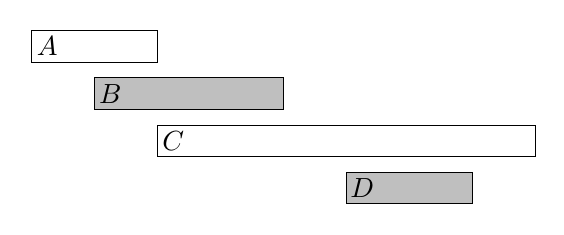
\begin{tikzpicture}[scale=.4]
  \begin{scope}
    \draw (2, 0) rectangle (6, -1);
    \draw[fill=lightgray] (4, -1.5) rectangle (10, -2.5);
    \draw (6, -3) rectangle (18, -4);
    \draw[fill=lightgray] (12, -4.5) rectangle (16, -5.5);
    \node at (2.5,-0.5) {$A$};
    \node at (4.5,-2) {$B$};
    \node at (6.5,-3.5) {$C$};
    \node at (12.5,-5) {$D$};
  \end{scope}
\end{tikzpicture}
\end{center}

可以为这个问题设计多种贪心算法，但哪一种在所有情况下都正确？

\subsubsection*{算法一}

第一种想法是选择尽可能\emph{短}的活动。在示例中，该算法选择如下活动：
\begin{center}
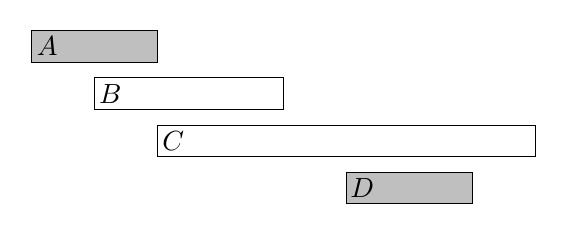
\begin{tikzpicture}[scale=.4]
  \begin{scope}
    \draw[fill=lightgray] (2, 0) rectangle (6, -1);
    \draw (4, -1.5) rectangle (10, -2.5);
    \draw (6, -3) rectangle (18, -4);
    \draw[fill=lightgray] (12, -4.5) rectangle (16, -5.5);
    \node at (2.5,-0.5) {$A$};
    \node at (4.5,-2) {$B$};
    \node at (6.5,-3.5) {$C$};
    \node at (12.5,-5) {$D$};
  \end{scope}
\end{tikzpicture}
\end{center}

然而，选择短活动并不总是正确的策略。例如，该算法在下列情形中会失败：
\begin{center}
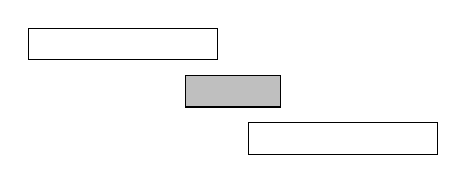
\begin{tikzpicture}[scale=.4]
  \begin{scope}
    \draw (1, 0) rectangle (7, -1);
    \draw[fill=lightgray] (6, -1.5) rectangle (9, -2.5);
    \draw (8, -3) rectangle (14, -4);
  \end{scope}
\end{tikzpicture}
\end{center}
如果选择短活动，就只能选择一个活动；但实际上两个长活动可以同时选取。

\subsubsection*{算法二}

另一种想法是始终选择可以选取且\emph{开始}得尽可能\emph{早}的下一个活动。该算法选择如下活动：
\begin{center}
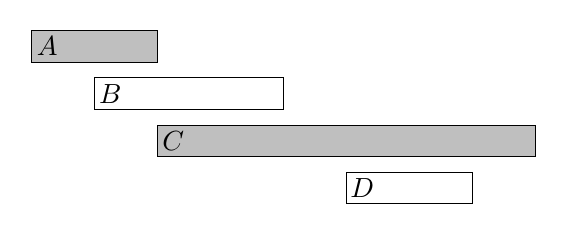
\begin{tikzpicture}[scale=.4]
  \begin{scope}
    \draw[fill=lightgray] (2, 0) rectangle (6, -1);
    \draw (4, -1.5) rectangle (10, -2.5);
    \draw[fill=lightgray] (6, -3) rectangle (18, -4);
    \draw (12, -4.5) rectangle (16, -5.5);
    \node at (2.5,-0.5) {$A$};
    \node at (4.5,-2) {$B$};
    \node at (6.5,-3.5) {$C$};
    \node at (12.5,-5) {$D$};
  \end{scope}
\end{tikzpicture}
\end{center}

然而，这个算法同样存在反例。例如，在下列情形中，算法只会选择一个活动：
\begin{center}
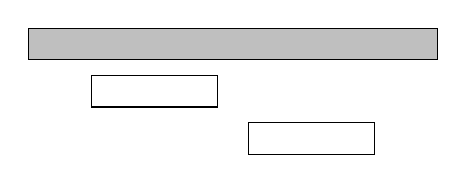
\begin{tikzpicture}[scale=.4]
  \begin{scope}
    \draw[fill=lightgray] (1, 0) rectangle (14, -1);
    \draw (3, -1.5) rectangle (7, -2.5);
    \draw (8, -3) rectangle (12, -4);
  \end{scope}
\end{tikzpicture}
\end{center}
如果选择第一个活动，就无法再选择任何其他活动；但实际上可以选择另外两个活动。

\subsubsection*{算法三}

第三种想法是始终选择可以选取且\emph{结束}得尽可能\emph{早}的下一个活动。该算法选择如下活动：
\begin{center}
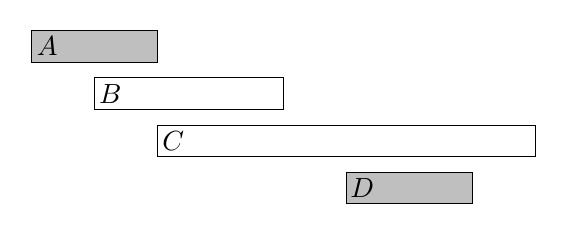
\begin{tikzpicture}[scale=.4]
  \begin{scope}
    \draw[fill=lightgray] (2, 0) rectangle (6, -1);
    \draw (4, -1.5) rectangle (10, -2.5);
    \draw (6, -3) rectangle (18, -4);
    \draw[fill=lightgray] (12, -4.5) rectangle (16, -5.5);
    \node at (2.5,-0.5) {$A$};
    \node at (4.5,-2) {$B$};
    \node at (6.5,-3.5) {$C$};
    \node at (12.5,-5) {$D$};
  \end{scope}
\end{tikzpicture}
\end{center}

事实证明，该算法\emph{总是}产生最优解。这是因为，首先选择结束时间最早的活动总是最优选择。之后继续用同样的策略选择下一个活动仍是最优的，如此反复，直到不能再选择活动。

证明该算法的一种方式，是考虑首先选择一个比最早结束活动结束得更晚的活动会怎样。此后可供选择的下一个活动数量至多与选择最早结束活动时相同。因此，选择结束更晚的活动绝不可能得到更好的解，贪心算法是正确的。

\section{任务与截止时间}

现在考虑一个问题：给定 $n$ 个任务及其持续时间和截止时间，需要选择执行任务的顺序。对每个任务，可获得 $d-x$ 分，其中 $d$ 是任务的截止时间，$x$ 是完成该任务的时刻。能够得到的最大总分是多少？

例如，设任务如下：
\begin{center}
\begin{tabular}{lll}
任务 & 持续时间 & 截止时间 \\
\hline
$A$ & 4 & 2 \\
$B$ & 3 & 5 \\
$C$ & 2 & 7 \\
$D$ & 4 & 5 \\
\end{tabular}
\end{center}
此时，一种最优任务安排如下：
\begin{center}
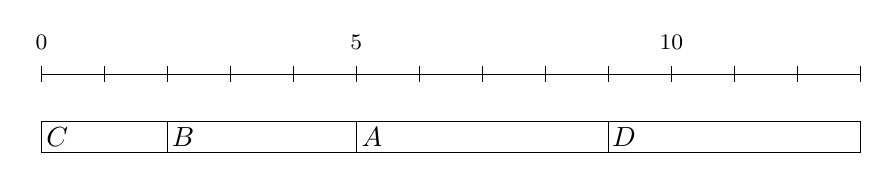
\begin{tikzpicture}[scale=.4]
  \begin{scope}
    \draw (0, 0) rectangle (4, -1);
    \draw (4, 0) rectangle (10, -1);
    \draw (10, 0) rectangle (18, -1);
    \draw (18, 0) rectangle (26, -1);
    \node at (0.5,-0.5) {$C$};
    \node at (4.5,-0.5) {$B$};
    \node at (10.5,-0.5) {$A$};
    \node at (18.5,-0.5) {$D$};

    \draw (0,1.5) -- (26,1.5);
    \foreach \i in {0,2,...,26}
    {
        \draw (\i,1.25) -- (\i,1.75);
    }
    \footnotesize
    \node at (0,2.5) {0};
    \node at (10,2.5) {5};
    \node at (20,2.5) {10};

  \end{scope}
\end{tikzpicture}
\end{center}
在这个解中，$C$ 得 5 分，$B$ 得 0 分，$A$ 得 $-7$ 分，$D$ 得 $-8$ 分，因此总分为 $-10$。

令人意外的是，该问题的最优解完全不依赖截止时间；正确的贪心策略只是按持续时间递增的顺序执行任务。原因在于，若连续执行的两个任务中前一个耗时更长，交换二者就能得到更好的解。例如，考虑如下安排：
\begin{center}
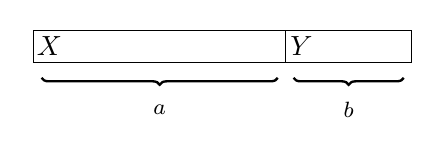
\begin{tikzpicture}[scale=.4]
  \begin{scope}
    \draw (0, 0) rectangle (8, -1);
    \draw (8, 0) rectangle (12, -1);
    \node at (0.5,-0.5) {$X$};
    \node at (8.5,-0.5) {$Y$};

\draw [decoration={brace}, decorate, line width=0.3mm] (7.75,-1.5) -- (0.25,-1.5);
\draw [decoration={brace}, decorate, line width=0.3mm] (11.75,-1.5) -- (8.25,-1.5);

\footnotesize
\node at (4,-2.5) {$a$};
\node at (10,-2.5) {$b$};

  \end{scope}
\end{tikzpicture}
\end{center}
这里 $a>b$，因此应交换两个任务：
\begin{center}
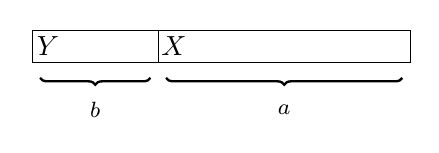
\begin{tikzpicture}[scale=.4]
  \begin{scope}
    \draw (0, 0) rectangle (4, -1);
    \draw (4, 0) rectangle (12, -1);
    \node at (0.5,-0.5) {$Y$};
    \node at (4.5,-0.5) {$X$};

\draw [decoration={brace}, decorate, line width=0.3mm] (3.75,-1.5) -- (0.25,-1.5);
\draw [decoration={brace}, decorate, line width=0.3mm] (11.75,-1.5) -- (4.25,-1.5);

\footnotesize
\node at (2,-2.5) {$b$};
\node at (8,-2.5) {$a$};

  \end{scope}
\end{tikzpicture}
\end{center}
现在，$X$ 少得 $b$ 分，$Y$ 多得 $a$ 分，所以总分增加 $a-b>0$。在最优解中，任意两个相邻任务都必须是较短任务排在较长任务之前。因此，任务必须按持续时间排序后执行。

\section{最小化总和}

接下来考虑一个问题：给定 $n$ 个数 $a_1,a_2,\ldots,a_n$，需要找到一个值 $x$，使下式最小：
\[|a_1-x|^c+|a_2-x|^c+\cdots+|a_n-x|^c.\]
我们重点讨论 $c=1$ 和 $c=2$ 两种情形。

\subsubsection{$c=1$ 的情形}

此时需要最小化
\[|a_1-x|+|a_2-x|+\cdots+|a_n-x|.\]
例如，如果这些数为 $[1,2,9,2,6]$，最优选择是 $x=2$，得到
\[
|1-2|+|2-2|+|9-2|+|2-2|+|6-2|=12.
\]
一般而言，$x$ 的最优选择是这些数的\key{中位数}，即排序后位于中间的数。例如，列表 $[1,2,9,2,6]$ 排序后为 $[1,2,2,6,9]$，所以中位数是 2。

中位数是最优选择，因为当 $x$ 小于中位数时，增大 $x$ 会使总和减小；当 $x$ 大于中位数时，减小 $x$ 会使总和减小。因此，最优解是令 $x$ 等于中位数。若 $n$ 为偶数而存在两个中位数，则这两个中位数及其之间的所有值都是最优选择。

\subsubsection{$c=2$ 的情形}

此时需要最小化
\[(a_1-x)^2+(a_2-x)^2+\cdots+(a_n-x)^2.\]
例如，如果这些数为 $[1,2,9,2,6]$，最优选择是 $x=4$，得到
\[
(1-4)^2+(2-4)^2+(9-4)^2+(2-4)^2+(6-4)^2=46.
\]
一般而言，$x$ 的最优选择是这些数的\key{平均数}。示例中的平均数为 $(1+2+9+2+6)/5=4$。将总和写成下式即可推导出这一结论：
\[
nx^2 - 2x(a_1+a_2+\cdots+a_n) + (a_1^2+a_2^2+\cdots+a_n^2)
\]
最后一部分与 $x$ 无关，因此可以忽略。其余部分构成函数 $nx^2-2xs$，其中 $s=a_1+a_2+\cdots+a_n$。这是一个开口向上的抛物线，两个零点为 $x=0$ 和 $x=2s/n$，最小值在两零点的平均位置 $x=s/n$ 处，也就是 $a_1,a_2,\ldots,a_n$ 的平均数。

\section{数据压缩}

\index{data compression}
\index{binary code}
\index{codeword}

\key{二进制编码}为字符串中的每个字符分配一个由比特组成的\key{码字}。将每个字符替换为对应码字，就可以用二进制编码\emph{压缩}字符串。例如，下列二进制编码为字符 \texttt{A}--\texttt{D} 分配码字：
\begin{center}
\begin{tabular}{rr}
字符 & 码字 \\
\hline
\texttt{A} & 00 \\
\texttt{B} & 01 \\
\texttt{C} & 10 \\
\texttt{D} & 11 \\
\end{tabular}
\end{center}
这是一种\key{定长编码}，即每个码字的长度都相同。例如，可以如下压缩字符串 \texttt{AABACDACA}：
\[00\,00\,01\,00\,10\,11\,00\,10\,00\]
使用这种编码，压缩后的字符串长 18 比特。不过，若使用码字长度可以不同的\key{变长编码}，还能进一步压缩：为频繁出现的字符分配短码字，为很少出现的字符分配长码字。事实证明，上述字符串的一种\key{最优}编码如下：
\begin{center}
\begin{tabular}{rr}
字符 & 码字 \\
\hline
\texttt{A} & 0 \\
\texttt{B} & 110 \\
\texttt{C} & 10 \\
\texttt{D} & 111 \\
\end{tabular}
\end{center}
最优编码产生的压缩字符串尽可能短。此时使用最优编码得到的压缩字符串为
\[0\,0\,110\,0\,10\,111\,0\,10\,0,\]
因此只需 15 比特而非 18 比特。借助更好的编码，压缩字符串节省了 3 比特。

要求任意码字都不能是另一码字的前缀。例如，编码中不能同时包含码字 10 和 1011。这是因为我们希望能够从压缩字符串还原原字符串；如果一个码字可以是另一个码字的前缀，就不一定能够做到这一点。例如，下列编码是\emph{无效的}：
\begin{center}
\begin{tabular}{rr}
字符 & 码字 \\
\hline
\texttt{A} & 10 \\
\texttt{B} & 11 \\
\texttt{C} & 1011 \\
\texttt{D} & 111 \\
\end{tabular}
\end{center}
使用这种编码，无法判断压缩字符串 1011 对应字符串 \texttt{AB} 还是字符串 \texttt{C}。

\index{Huffman coding}

\subsubsection{Huffman 编码}

\key{Huffman 编码}\footnote{D. A. Huffman 在完成大学课程作业时发现了这种方法，并于 1952 年发表该算法 \cite{huf52}。}是一种为给定字符串构造最优压缩编码的贪心算法。算法根据字符串中各字符的频率建立一棵二叉树；沿根结点到相应结点的路径即可读出每个字符的码字。向左移动对应比特 0，向右移动对应比特 1。

初始时，字符串中的每个字符由一个结点表示，结点权值是该字符在字符串中的出现次数。此后每一步合并权值最小的两个结点，创建一个新结点，其权值为原来两个结点的权值之和。不断重复，直到所有结点都被合并。

下面来看 Huffman 编码如何为字符串 \texttt{AABACDACA} 构造最优编码。初始时有四个结点，分别对应字符串中的四种字符：

\begin{center}
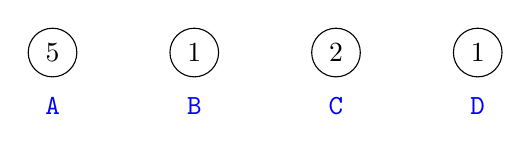
\begin{tikzpicture}[scale=0.9]
\node[draw, circle] (1) at (0,0) {$5$};
\node[draw, circle] (2) at (2,0) {$1$};
\node[draw, circle] (3) at (4,0) {$2$};
\node[draw, circle] (4) at (6,0) {$1$};

\node[color=blue] at (0,-0.75) {\texttt{A}};
\node[color=blue] at (2,-0.75) {\texttt{B}};
\node[color=blue] at (4,-0.75) {\texttt{C}};
\node[color=blue] at (6,-0.75) {\texttt{D}};

%\path[draw,thick,-] (4) -- (5);
\end{tikzpicture}
\end{center}
表示字符 \texttt{A} 的结点权值为 5，因为 \texttt{A} 在字符串中出现了 5 次。其他权值也以同样方式计算。

第一步合并分别对应字符 \texttt{B} 和 \texttt{D} 的结点，二者权值均为 1。结果如下：
\begin{center}
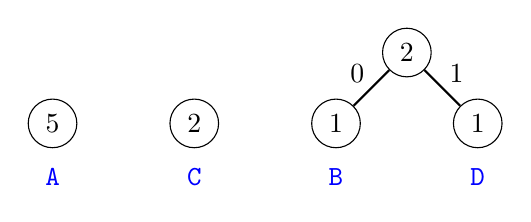
\begin{tikzpicture}[scale=0.9]
\node[draw, circle] (1) at (0,0) {$5$};
\node[draw, circle] (3) at (2,0) {$2$};
\node[draw, circle] (2) at (4,0) {$1$};
\node[draw, circle] (4) at (6,0) {$1$};
\node[draw, circle] (5) at (5,1) {$2$};

\node[color=blue] at (0,-0.75) {\texttt{A}};
\node[color=blue] at (2,-0.75) {\texttt{C}};
\node[color=blue] at (4,-0.75) {\texttt{B}};
\node[color=blue] at (6,-0.75) {\texttt{D}};

\node at (4.3,0.7) {0};
\node at (5.7,0.7) {1};

\path[draw,thick,-] (2) -- (5);
\path[draw,thick,-] (4) -- (5);
\end{tikzpicture}
\end{center}
之后，合并两个权值为 2 的结点：
\begin{center}
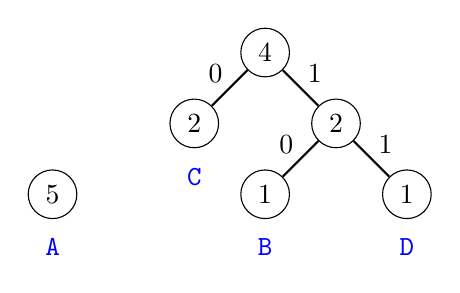
\begin{tikzpicture}[scale=0.9]
\node[draw, circle] (1) at (1,0) {$5$};
\node[draw, circle] (3) at (3,1) {$2$};
\node[draw, circle] (2) at (4,0) {$1$};
\node[draw, circle] (4) at (6,0) {$1$};
\node[draw, circle] (5) at (5,1) {$2$};
\node[draw, circle] (6) at (4,2) {$4$};

\node[color=blue] at (1,-0.75) {\texttt{A}};
\node[color=blue] at (3,1-0.75) {\texttt{C}};
\node[color=blue] at (4,-0.75) {\texttt{B}};
\node[color=blue] at (6,-0.75) {\texttt{D}};

\node at (4.3,0.7) {0};
\node at (5.7,0.7) {1};
\node at (3.3,1.7) {0};
\node at (4.7,1.7) {1};

\path[draw,thick,-] (2) -- (5);
\path[draw,thick,-] (4) -- (5);
\path[draw,thick,-] (3) -- (6);
\path[draw,thick,-] (5) -- (6);
\end{tikzpicture}
\end{center}
最后，合并剩余的两个结点：
\begin{center}
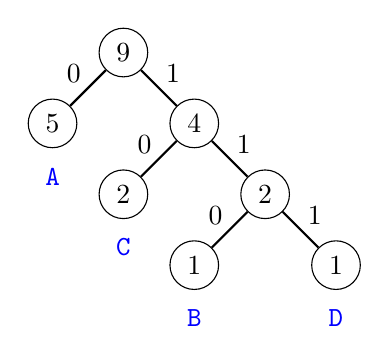
\begin{tikzpicture}[scale=0.9]
\node[draw, circle] (1) at (2,2) {$5$};
\node[draw, circle] (3) at (3,1) {$2$};
\node[draw, circle] (2) at (4,0) {$1$};
\node[draw, circle] (4) at (6,0) {$1$};
\node[draw, circle] (5) at (5,1) {$2$};
\node[draw, circle] (6) at (4,2) {$4$};
\node[draw, circle] (7) at (3,3) {$9$};

\node[color=blue] at (2,2-0.75) {\texttt{A}};
\node[color=blue] at (3,1-0.75) {\texttt{C}};
\node[color=blue] at (4,-0.75) {\texttt{B}};
\node[color=blue] at (6,-0.75) {\texttt{D}};

\node at (4.3,0.7) {0};
\node at (5.7,0.7) {1};
\node at (3.3,1.7) {0};
\node at (4.7,1.7) {1};
\node at (2.3,2.7) {0};
\node at (3.7,2.7) {1};

\path[draw,thick,-] (2) -- (5);
\path[draw,thick,-] (4) -- (5);
\path[draw,thick,-] (3) -- (6);
\path[draw,thick,-] (5) -- (6);
\path[draw,thick,-] (1) -- (7);
\path[draw,thick,-] (6) -- (7);
\end{tikzpicture}
\end{center}

现在所有结点都已进入树中，编码构造完毕。可以从树中读出下列码字：
\begin{center}
\begin{tabular}{rr}
字符 & 码字 \\
\hline
\texttt{A} & 0 \\
\texttt{B} & 110 \\
\texttt{C} & 10 \\
\texttt{D} & 111 \\
\end{tabular}
\end{center}
